% Lienzo de modelo de negocio (Osterwalder y Pigneur) de Allocia.
\begin{figure}[ht]\centering
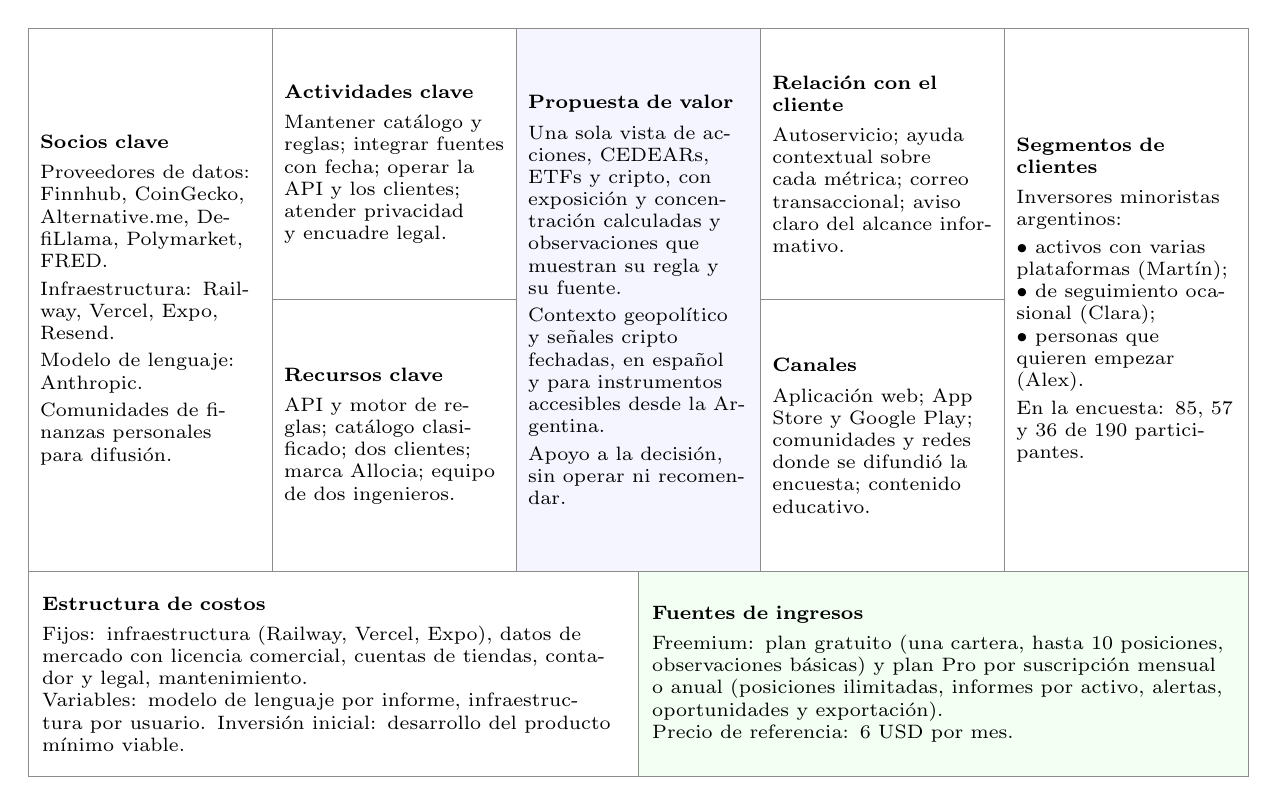
\begin{tikzpicture}[font=\scriptsize,
  blk/.style={draw=black!45,fill=white,inner sep=4pt,align=left,anchor=north west},
  t/.style={font=\scriptsize\bfseries}]
\def\w{3.1}\def\hh{6.9}\def\hl{2.6}
\node[blk,minimum width=\w cm,minimum height=\hh cm,text width=2.8cm] at (0,0) {\textbf{Socios clave}\\[3pt]Proveedores de datos: Finnhub, CoinGecko, Alternative.me, DefiLlama, Polymarket, FRED.\\[2pt]Infraestructura: Railway, Vercel, Expo, Resend.\\[2pt]Modelo de lenguaje: Anthropic.\\[2pt]Comunidades de finanzas personales para difusión.};
\node[blk,minimum width=\w cm,minimum height=3.45cm,text width=2.8cm] at (\w,0) {\textbf{Actividades clave}\\[3pt]Mantener catálogo y reglas; integrar fuentes con fecha; operar la API y los clientes; atender privacidad y encuadre legal.};
\node[blk,minimum width=\w cm,minimum height=3.45cm,text width=2.8cm] at (\w,-3.45) {\textbf{Recursos clave}\\[3pt]API y motor de reglas; catálogo clasificado; dos clientes; marca Allocia; equipo de dos ingenieros.};
\node[blk,minimum width=\w cm,minimum height=\hh cm,text width=2.8cm,fill=blue!4] at (2*\w,0) {\textbf{Propuesta de valor}\\[3pt]Una sola vista de acciones, CEDEARs, ETFs y cripto, con exposición y concentración calculadas y observaciones que muestran su regla y su fuente.\\[2pt]Contexto geopolítico y señales cripto fechadas, en español y para instrumentos accesibles desde la Argentina.\\[2pt]Apoyo a la decisión, sin operar ni recomendar.};
\node[blk,minimum width=\w cm,minimum height=3.45cm,text width=2.8cm] at (3*\w,0) {\textbf{Relación con el cliente}\\[3pt]Autoservicio; ayuda contextual sobre cada métrica; correo transaccional; aviso claro del alcance informativo.};
\node[blk,minimum width=\w cm,minimum height=3.45cm,text width=2.8cm] at (3*\w,-3.45) {\textbf{Canales}\\[3pt]Aplicación web; App Store y Google Play; comunidades y redes donde se difundió la encuesta; contenido educativo.};
\node[blk,minimum width=\w cm,minimum height=\hh cm,text width=2.8cm] at (4*\w,0) {\textbf{Segmentos de clientes}\\[3pt]Inversores minoristas argentinos:\\[2pt]$\bullet$ activos con varias plataformas (Martín);\\$\bullet$ de seguimiento ocasional (Clara);\\$\bullet$ personas que quieren empezar (Alex).\\[2pt]En la encuesta: 85, 57 y 36 de 190 participantes.};
\node[blk,minimum width=2.5*\w cm,minimum height=\hl cm,text width=7.4cm] at (0,-\hh) {\textbf{Estructura de costos}\\[3pt]Fijos: infraestructura (Railway, Vercel, Expo), datos de mercado con licencia comercial, cuentas de tiendas, contador y legal, mantenimiento.\\Variables: modelo de lenguaje por informe, infraestructura por usuario. Inversión inicial: desarrollo del producto mínimo viable.};
\node[blk,minimum width=2.5*\w cm,minimum height=\hl cm,text width=7.4cm,fill=green!5] at (2.5*\w,-\hh) {\textbf{Fuentes de ingresos}\\[3pt]Freemium: plan gratuito (una cartera, hasta 10 posiciones, observaciones básicas) y plan Pro por suscripción mensual o anual (posiciones ilimitadas, informes por activo, alertas, oportunidades y exportación).\\Precio de referencia: 6 USD por mes.};
\end{tikzpicture}
\caption{Lienzo del modelo de negocio de Allocia. Fuente: elaboración propia a partir del lienzo de modelo de negocio \parencite{Osterwalder2010}.}\label{fig:canvas}
\end{figure}
